\documentclass[1p]{elsarticle_modified}
%\bibliographystyle{elsarticle-num}

%\usepackage[colorlinks]{hyperref}
%\usepackage{abbrmath_seonhwa} %\Abb, \Ascr, \Acal ,\Abf, \Afrak
\usepackage{amsfonts}
\usepackage{amssymb}
\usepackage{amsmath}
\usepackage{amsthm}
\usepackage{scalefnt}
\usepackage{amsbsy}
\usepackage{kotex}
\usepackage{caption}
\usepackage{subfig}
\usepackage{color}
\usepackage{graphicx}
\usepackage{xcolor} %% white, black, red, green, blue, cyan, magenta, yellow
\usepackage{float}
\usepackage{setspace}
\usepackage{hyperref}

\usepackage{tikz}
\usetikzlibrary{arrows}

\usepackage{multirow}
\usepackage{array} % fixed length table
\usepackage{hhline}

%%%%%%%%%%%%%%%%%%%%%
\makeatletter
\renewcommand*\env@matrix[1][\arraystretch]{%
	\edef\arraystretch{#1}%
	\hskip -\arraycolsep
	\let\@ifnextchar\new@ifnextchar
	\array{*\c@MaxMatrixCols c}}
\makeatother %https://tex.stackexchange.com/questions/14071/how-can-i-increase-the-line-spacing-in-a-matrix
%%%%%%%%%%%%%%%

\usepackage[normalem]{ulem}

\newcommand{\msout}[1]{\ifmmode\text{\sout{\ensuremath{#1}}}\else\sout{#1}\fi}
%SOURCE: \msout is \stkout macro in https://tex.stackexchange.com/questions/20609/strikeout-in-math-mode

\newcommand{\cancel}[1]{
	\ifmmode
	{\color{red}\msout{#1}}
	\else
	{\color{red}\sout{#1}}
	\fi
}

\newcommand{\add}[1]{
	{\color{blue}\uwave{#1}}
}

\newcommand{\replace}[2]{
	\ifmmode
	{\color{red}\msout{#1}}{\color{blue}\uwave{#2}}
	\else
	{\color{red}\sout{#1}}{\color{blue}\uwave{#2}}
	\fi
}

\newcommand{\Sol}{\mathcal{S}} %segment
\newcommand{\D}{D} %diagram
\newcommand{\A}{\mathcal{A}} %arc


%%%%%%%%%%%%%%%%%%%%%%%%%%%%%5 test

\def\sl{\operatorname{\textup{SL}}(2,\Cbb)}
\def\psl{\operatorname{\textup{PSL}}(2,\Cbb)}
\def\quan{\mkern 1mu \triangleright \mkern 1mu}

\theoremstyle{definition}
\newtheorem{thm}{Theorem}[section]
\newtheorem{prop}[thm]{Proposition}
\newtheorem{lem}[thm]{Lemma}
\newtheorem{ques}[thm]{Question}
\newtheorem{cor}[thm]{Corollary}
\newtheorem{defn}[thm]{Definition}
\newtheorem{exam}[thm]{Example}
\newtheorem{rmk}[thm]{Remark}
\newtheorem{alg}[thm]{Algorithm}

\newcommand{\I}{\sqrt{-1}}
\begin{document}

%\begin{frontmatter}
%
%\title{Boundary parabolic representations of knots up to 8 crossings}
%
%%% Group authors per affiliation:
%\author{Yunhi Cho} 
%\address{Department of Mathematics, University of Seoul, Seoul, Korea}
%\ead{yhcho@uos.ac.kr}
%
%
%\author{Seonhwa Kim} %\fnref{s_kim}}
%\address{Center for Geometry and Physics, Institute for Basic Science, Pohang, 37673, Korea}
%\ead{ryeona17@ibs.re.kr}
%
%\author{Hyuk Kim}
%\address{Department of Mathematical Sciences, Seoul National University, Seoul 08826, Korea}
%\ead{hyukkim@snu.ac.kr}
%
%\author{Seokbeom Yoon}
%\address{Department of Mathematical Sciences, Seoul National University, Seoul, 08826,  Korea}
%\ead{sbyoon15@snu.ac.kr}
%
%\begin{abstract}
%We find all boundary parabolic representation of knots up to 8 crossings.
%
%\end{abstract}
%\begin{keyword}
%    \MSC[2010] 57M25 
%\end{keyword}
%
%\end{frontmatter}

%\linenumbers
%\tableofcontents
%
\newcommand\colored[1]{\textcolor{white}{\rule[-0.35ex]{0.8em}{1.4ex}}\kern-0.8em\color{red} #1}%
%\newcommand\colored[1]{\textcolor{white}{ #1}\kern-2.17ex	\textcolor{white}{ #1}\kern-1.81ex	\textcolor{white}{ #1}\kern-2.15ex\color{red}#1	}

{\Large $\underline{11a_{51}~(K11a_{51})}$}

\setlength{\tabcolsep}{10pt}
\renewcommand{\arraystretch}{1.6}
\vspace{1cm}\begin{tabular}{m{100pt}>{\centering\arraybackslash}m{274pt}}
\multirow{5}{120pt}{
	\centering
	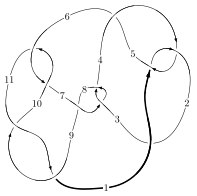
\includegraphics[width=112pt]{../../../GIT/diagram.site/Diagrams/png/300_11a_51.png}\\
\ \ \ A knot diagram\footnotemark}&
\allowdisplaybreaks
\textbf{Linearized knot diagam} \\
\cline{2-2}
 &
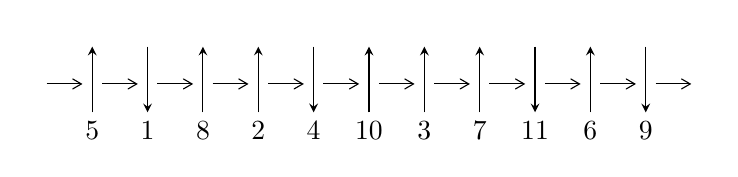
\begin{tikzpicture}[x=20pt, y=17pt]
	% nodes
	\node (C0) at (0, 0) {};
	\node (C1) at (1, 0) {};
	\node (C1U) at (1, +1) {};
	\node (C1D) at (1, -1) {5};

	\node (C2) at (2, 0) {};
	\node (C2U) at (2, +1) {};
	\node (C2D) at (2, -1) {1};

	\node (C3) at (3, 0) {};
	\node (C3U) at (3, +1) {};
	\node (C3D) at (3, -1) {8};

	\node (C4) at (4, 0) {};
	\node (C4U) at (4, +1) {};
	\node (C4D) at (4, -1) {2};

	\node (C5) at (5, 0) {};
	\node (C5U) at (5, +1) {};
	\node (C5D) at (5, -1) {4};

	\node (C6) at (6, 0) {};
	\node (C6U) at (6, +1) {};
	\node (C6D) at (6, -1) {10};

	\node (C7) at (7, 0) {};
	\node (C7U) at (7, +1) {};
	\node (C7D) at (7, -1) {3};

	\node (C8) at (8, 0) {};
	\node (C8U) at (8, +1) {};
	\node (C8D) at (8, -1) {7};

	\node (C9) at (9, 0) {};
	\node (C9U) at (9, +1) {};
	\node (C9D) at (9, -1) {11};

	\node (C10) at (10, 0) {};
	\node (C10U) at (10, +1) {};
	\node (C10D) at (10, -1) {6};

	\node (C11) at (11, 0) {};
	\node (C11U) at (11, +1) {};
	\node (C11D) at (11, -1) {9};
	\node (C12) at (12, 0) {};

	% arrows
	\draw[->,>={angle 60}]
	(C0) edge (C1) (C1) edge (C2) (C2) edge (C3) (C3) edge (C4) (C4) edge (C5) (C5) edge (C6) (C6) edge (C7) (C7) edge (C8) (C8) edge (C9) (C9) edge (C10) (C10) edge (C11) (C11) edge (C12) ;	\draw[->,>=stealth]
	(C1D) edge (C1U) (C2U) edge (C2D) (C3D) edge (C3U) (C4D) edge (C4U) (C5U) edge (C5D) (C6D) edge (C6U) (C7D) edge (C7U) (C8D) edge (C8U) (C9U) edge (C9D) (C10D) edge (C10U) (C11U) edge (C11D) ;
	\end{tikzpicture} \\
\hhline{~~} \\& 
\textbf{Solving Sequence} \\ \cline{2-2} 
 &
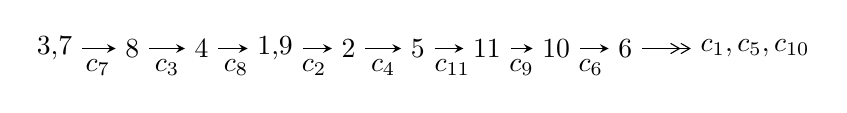
\begin{tikzpicture}[x=25pt, y=7pt]
	% node
	\node (A0) at (-1/8, 0) {3,7};
	\node (A1) at (1, 0) {8};
	\node (A2) at (2, 0) {4};
	\node (A3) at (49/16, 0) {1,9};
	\node (A4) at (33/8, 0) {2};
	\node (A5) at (41/8, 0) {5};
	\node (A6) at (49/8, 0) {11};
	\node (A7) at (57/8, 0) {10};
	\node (A8) at (65/8, 0) {6};
	\node (C1) at (1/2, -1) {$c_{7}$};
	\node (C2) at (3/2, -1) {$c_{3}$};
	\node (C3) at (5/2, -1) {$c_{8}$};
	\node (C4) at (29/8, -1) {$c_{2}$};
	\node (C5) at (37/8, -1) {$c_{4}$};
	\node (C6) at (45/8, -1) {$c_{11}$};
	\node (C7) at (53/8, -1) {$c_{9}$};
	\node (C8) at (61/8, -1) {$c_{6}$};
	\node (A9) at (10, 0) {$c_{1},c_{5},c_{10}$};

	% edge
	\draw[->,>=stealth]	
	(A0) edge (A1) (A1) edge (A2) (A2) edge (A3) (A3) edge (A4) (A4) edge (A5) (A5) edge (A6) (A6) edge (A7) (A7) edge (A8) ;
	\draw[->>,>={angle 60}]	
	(A8) edge (A9);
\end{tikzpicture} \\ 

\end{tabular} \\

\footnotetext{
The image of knot diagram is generated by the software ``\textbf{Draw programme}" developed by Andrew Bartholomew(\url{http://www.layer8.co.uk/maths/draw/index.htm\#Running-draw}), where we modified some parts for our purpose(\url{https://github.com/CATsTAILs/LinksPainter}).
}\phantom \\ \newline 
\centering \textbf{Ideals for irreducible components\footnotemark of $X_{\text{par}}$} 
 
\begin{align*}
I^u_{1}&=\langle 
-5 u^{14}+23 u^{13}+\cdots+4 b-28,\\
\phantom{I^u_{1}}&\phantom{= \langle  }2 u^{14}-7 u^{13}+9 u^{12}+6 u^{11}-33 u^{10}+42 u^9-6 u^8-42 u^7+53 u^6-19 u^5-7 u^4+6 u^3+11 u^2+4 a-10 u+2,\\
\phantom{I^u_{1}}&\phantom{= \langle  }u^{15}-5 u^{14}+10 u^{13}-5 u^{12}-18 u^{11}+44 u^{10}-40 u^9-3 u^8+49 u^7-55 u^6+26 u^5- u^4+2 u^3-12 u^2+12 u-4\rangle \\
I^u_{2}&=\langle 
2 u^{22} a+8 u^{22}+\cdots-4 a-16,\;-2 u^{21} a+7 u^{22}+\cdots+6 a-11,\;u^{23}+2 u^{22}+\cdots-5 u-2\rangle \\
\\
I^v_{1}&=\langle 
a,\;b^2- b+1,\;v+1\rangle \\
I^v_{2}&=\langle 
a,\;b- v,\;v^2- v+1\rangle \\
\end{align*}
\raggedright * 4 irreducible components of $\dim_{\mathbb{C}}=0$, with total 65 representations.\\
\footnotetext{All coefficients of polynomials are rational numbers. But the coefficients are sometimes approximated in decimal forms when there is not enough margin.}
\newpage
\renewcommand{\arraystretch}{1}
\centering \section*{I. $I^u_{1}= \langle -5 u^{14}+23 u^{13}+\cdots+4 b-28,\;2 u^{14}-7 u^{13}+\cdots+4 a+2,\;u^{15}-5 u^{14}+\cdots+12 u-4 \rangle$}
\flushleft \textbf{(i) Arc colorings}\\
\begin{tabular}{m{7pt} m{180pt} m{7pt} m{180pt} }
\flushright $a_{3}=$&$\begin{pmatrix}0\\u\end{pmatrix}$ \\
\flushright $a_{7}=$&$\begin{pmatrix}1\\0\end{pmatrix}$ \\
\flushright $a_{8}=$&$\begin{pmatrix}1\\- u^2\end{pmatrix}$ \\
\flushright $a_{4}=$&$\begin{pmatrix}u\\- u^3+u\end{pmatrix}$ \\
\flushright $a_{1}=$&$\begin{pmatrix}-\frac{1}{2} u^{14}+\frac{7}{4} u^{13}+\cdots+\frac{5}{2} u-\frac{1}{2}\\\frac{5}{4} u^{14}-\frac{23}{4} u^{13}+\cdots-\frac{27}{2} u+7\end{pmatrix}$ \\
\flushright $a_{9}=$&$\begin{pmatrix}- u^2+1\\- u^2\end{pmatrix}$ \\
\flushright $a_{2}=$&$\begin{pmatrix}-\frac{1}{4} u^{14}+u^{13}+\cdots+\frac{3}{2} u-\frac{1}{2}\\-\frac{1}{4} u^{14}+\frac{3}{4} u^{13}+\cdots- u^2+\frac{3}{2} u\end{pmatrix}$ \\
\flushright $a_{5}=$&$\begin{pmatrix}\frac{3}{4} u^{14}-4 u^{13}+\cdots-9 u+\frac{9}{2}\\\frac{7}{4} u^{14}-\frac{29}{4} u^{13}+\cdots-\frac{25}{2} u+5\end{pmatrix}$ \\
\flushright $a_{11}=$&$\begin{pmatrix}-\frac{5}{4} u^{14}+\frac{9}{2} u^{13}+\cdots+6 u-\frac{5}{2}\\-\frac{1}{4} u^{14}-\frac{1}{4} u^{13}+\cdots-\frac{9}{2} u+3\end{pmatrix}$ \\
\flushright $a_{10}=$&$\begin{pmatrix}-\frac{1}{2} u^{14}+\frac{7}{4} u^{13}+\cdots+2 u+\frac{1}{2}\\-\frac{1}{4} u^{14}+\frac{3}{4} u^{13}+\cdots-2 u^2+\frac{1}{2} u\end{pmatrix}$ \\
\flushright $a_{6}=$&$\begin{pmatrix}\frac{7}{4} u^{14}-\frac{15}{2} u^{13}+\cdots-16 u+\frac{15}{2}\\\frac{3}{4} u^{14}-\frac{11}{4} u^{13}+\cdots-\frac{11}{2} u+2\end{pmatrix}$\\ \flushright $a_{6}=$&$\begin{pmatrix}\frac{7}{4} u^{14}-\frac{15}{2} u^{13}+\cdots-16 u+\frac{15}{2}\\\frac{3}{4} u^{14}-\frac{11}{4} u^{13}+\cdots-\frac{11}{2} u+2\end{pmatrix}$\\&\end{tabular}
\flushleft \textbf{(ii) Obstruction class $= -1$}\\~\\
\flushleft \textbf{(iii) Cusp Shapes $= 13 u^{14}-58 u^{13}+91 u^{12}+9 u^{11}-253 u^{10}+402 u^9-196 u^8-247 u^7+488 u^6-328 u^5+45 u^4+37 u^3+59 u^2-114 u+58$}\\~\\
\newpage\renewcommand{\arraystretch}{1}
\flushleft \textbf{(iv) u-Polynomials at the component}\newline \\
\begin{tabular}{m{50pt}|m{274pt}}
Crossings & \hspace{64pt}u-Polynomials at each crossing \\
\hline $$\begin{aligned}c_{1},c_{4},c_{6}\\c_{10}\end{aligned}$$&$\begin{aligned}
&u^{15}+u^{14}+\cdots+2 u-1
\end{aligned}$\\
\hline $$\begin{aligned}c_{2},c_{5},c_{9}\\c_{11}\end{aligned}$$&$\begin{aligned}
&u^{15}+5 u^{14}+\cdots+18 u^2-1
\end{aligned}$\\
\hline $$\begin{aligned}c_{3},c_{7}\end{aligned}$$&$\begin{aligned}
&u^{15}-5 u^{14}+\cdots+12 u-4
\end{aligned}$\\
\hline $$\begin{aligned}c_{8}\end{aligned}$$&$\begin{aligned}
&u^{15}-5 u^{14}+\cdots+48 u-16
\end{aligned}$\\
\hline
\end{tabular}\\~\\
\newpage\renewcommand{\arraystretch}{1}
\flushleft \textbf{(v) Riley Polynomials at the component}\newline \\
\begin{tabular}{m{50pt}|m{274pt}}
Crossings & \hspace{64pt}Riley Polynomials at each crossing \\
\hline $$\begin{aligned}c_{1},c_{4},c_{6}\\c_{10}\end{aligned}$$&$\begin{aligned}
&y^{15}+5 y^{14}+\cdots+18 y^2-1
\end{aligned}$\\
\hline $$\begin{aligned}c_{2},c_{5},c_{9}\\c_{11}\end{aligned}$$&$\begin{aligned}
&y^{15}+13 y^{14}+\cdots+36 y-1
\end{aligned}$\\
\hline $$\begin{aligned}c_{3},c_{7}\end{aligned}$$&$\begin{aligned}
&y^{15}-5 y^{14}+\cdots+48 y-16
\end{aligned}$\\
\hline $$\begin{aligned}c_{8}\end{aligned}$$&$\begin{aligned}
&y^{15}+3 y^{14}+\cdots-1024 y-256
\end{aligned}$\\
\hline
\end{tabular}\\~\\
\newpage\flushleft \textbf{(vi) Complex Volumes and Cusp Shapes}
$$\begin{array}{c|c|c}  
\text{Solutions to }I^u_{1}& \I (\text{vol} + \sqrt{-1}CS) & \text{Cusp shape}\\
 \hline 
\begin{aligned}
u &= \phantom{-}0.297110 + 1.013620 I \\
a &= -0.987350 - 0.311397 I \\
b &= -0.738671 + 0.490241 I\end{aligned}
 & \phantom{-}3.26489 + 2.24335 I & \phantom{-}7.04256 - 3.44027 I \\ \hline\begin{aligned}
u &= \phantom{-}0.297110 - 1.013620 I \\
a &= -0.987350 + 0.311397 I \\
b &= -0.738671 - 0.490241 I\end{aligned}
 & \phantom{-}3.26489 - 2.24335 I & \phantom{-}7.04256 + 3.44027 I \\ \hline\begin{aligned}
u &= \phantom{-}0.843039 + 0.715120 I \\
a &= \phantom{-}0.718904 - 0.735528 I \\
b &= -0.47287 - 1.47924 I\end{aligned}
 & -6.27477 + 2.71677 I & -5.40032 - 3.41816 I \\ \hline\begin{aligned}
u &= \phantom{-}0.843039 - 0.715120 I \\
a &= \phantom{-}0.718904 + 0.735528 I \\
b &= -0.47287 + 1.47924 I\end{aligned}
 & -6.27477 - 2.71677 I & -5.40032 + 3.41816 I \\ \hline\begin{aligned}
u &= \phantom{-}0.528547 + 1.045590 I \\
a &= \phantom{-}1.235390 + 0.154632 I \\
b &= \phantom{-}0.915557 - 0.882680 I\end{aligned}
 & \phantom{-}1.75577 - 8.71874 I & \phantom{-}3.93323 + 7.24615 I \\ \hline\begin{aligned}
u &= \phantom{-}0.528547 - 1.045590 I \\
a &= \phantom{-}1.235390 - 0.154632 I \\
b &= \phantom{-}0.915557 + 0.882680 I\end{aligned}
 & \phantom{-}1.75577 + 8.71874 I & \phantom{-}3.93323 - 7.24615 I \\ \hline\begin{aligned}
u &= -0.548950 + 0.445559 I \\
a &= -0.294279 - 0.663565 I \\
b &= -0.232624 - 0.217433 I\end{aligned}
 & -1.34006 - 1.53790 I & -1.51731 + 5.00908 I \\ \hline\begin{aligned}
u &= -0.548950 - 0.445559 I \\
a &= -0.294279 + 0.663565 I \\
b &= -0.232624 + 0.217433 I\end{aligned}
 & -1.34006 + 1.53790 I & -1.51731 - 5.00908 I \\ \hline\begin{aligned}
u &= \phantom{-}0.700518\phantom{ +0.000000I} \\
a &= -0.240121\phantom{ +0.000000I} \\
b &= \phantom{-}0.561665\phantom{ +0.000000I}\end{aligned}
 & \phantom{-}0.940705\phantom{ +0.000000I} & \phantom{-}11.2760\phantom{ +0.000000I} \\ \hline\begin{aligned}
u &= \phantom{-}1.194600 + 0.597734 I \\
a &= \phantom{-}0.209836 + 0.830578 I \\
b &= \phantom{-}1.56955 + 0.92220 I\end{aligned}
 & \phantom{-}6.11311 + 3.45523 I & \phantom{-}8.74146 - 0.79948 I\\
 \hline 
 \end{array}$$\newpage$$\begin{array}{c|c|c}  
\text{Solutions to }I^u_{1}& \I (\text{vol} + \sqrt{-1}CS) & \text{Cusp shape}\\
 \hline 
\begin{aligned}
u &= \phantom{-}1.194600 - 0.597734 I \\
a &= \phantom{-}0.209836 - 0.830578 I \\
b &= \phantom{-}1.56955 - 0.92220 I\end{aligned}
 & \phantom{-}6.11311 - 3.45523 I & \phantom{-}8.74146 + 0.79948 I \\ \hline\begin{aligned}
u &= -1.338190 + 0.093539 I \\
a &= -0.043731 - 1.064360 I \\
b &= -0.043240 - 0.609135 I\end{aligned}
 & \phantom{-}9.46149 - 5.98215 I & \phantom{-}9.71265 + 5.53392 I \\ \hline\begin{aligned}
u &= -1.338190 - 0.093539 I \\
a &= -0.043731 + 1.064360 I \\
b &= -0.043240 + 0.609135 I\end{aligned}
 & \phantom{-}9.46149 + 5.98215 I & \phantom{-}9.71265 - 5.53392 I \\ \hline\begin{aligned}
u &= \phantom{-}1.173580 + 0.723559 I \\
a &= -0.218707 - 1.141120 I \\
b &= -1.77854 - 1.21305 I\end{aligned}
 & \phantom{-}3.8210 + 15.1159 I & \phantom{-}4.84980 - 10.19781 I \\ \hline\begin{aligned}
u &= \phantom{-}1.173580 - 0.723559 I \\
a &= -0.218707 + 1.141120 I \\
b &= -1.77854 + 1.21305 I\end{aligned}
 & \phantom{-}3.8210 - 15.1159 I & \phantom{-}4.84980 + 10.19781 I\\
 \hline 
 \end{array}$$\newpage\newpage\renewcommand{\arraystretch}{1}
\centering \section*{II. $I^u_{2}= \langle 2 u^{22} a+8 u^{22}+\cdots-4 a-16,\;-2 u^{21} a+7 u^{22}+\cdots+6 a-11,\;u^{23}+2 u^{22}+\cdots-5 u-2 \rangle$}
\flushleft \textbf{(i) Arc colorings}\\
\begin{tabular}{m{7pt} m{180pt} m{7pt} m{180pt} }
\flushright $a_{3}=$&$\begin{pmatrix}0\\u\end{pmatrix}$ \\
\flushright $a_{7}=$&$\begin{pmatrix}1\\0\end{pmatrix}$ \\
\flushright $a_{8}=$&$\begin{pmatrix}1\\- u^2\end{pmatrix}$ \\
\flushright $a_{4}=$&$\begin{pmatrix}u\\- u^3+u\end{pmatrix}$ \\
\flushright $a_{1}=$&$\begin{pmatrix}a\\- u^{22} a-4 u^{22}+\cdots+2 a+8\end{pmatrix}$ \\
\flushright $a_{9}=$&$\begin{pmatrix}- u^2+1\\- u^2\end{pmatrix}$ \\
\flushright $a_{2}=$&$\begin{pmatrix}\frac{1}{2} u^{22} a+\frac{3}{2} u^{22}+\cdots-6 u-\frac{7}{2}\\-\frac{7}{2} u^{22} a-\frac{5}{2} u^{22}+\cdots+8 a+8\end{pmatrix}$ \\
\flushright $a_{5}=$&$\begin{pmatrix}- u^{22} a-4 u^{22}+\cdots+a+8\\-\frac{1}{2} u^{22}-\frac{1}{2} u^{21}+\cdots+a u+\frac{3}{2} u\end{pmatrix}$ \\
\flushright $a_{11}=$&$\begin{pmatrix}-\frac{1}{2} u^{19}+2 u^{17}+\cdots+a-1\\- u^{22} a-\frac{7}{2} u^{22}+\cdots+2 a+7\end{pmatrix}$ \\
\flushright $a_{10}=$&$\begin{pmatrix}3 u^{22}+\frac{5}{2} u^{21}+\cdots-10 u-\frac{9}{2}\\\frac{7}{2} u^{22} a+\frac{5}{2} u^{22}+\cdots-7 a-6\end{pmatrix}$ \\
\flushright $a_{6}=$&$\begin{pmatrix}- u^{22} a-4 u^{22}+\cdots+a+8\\-\frac{1}{2} u^{22}-\frac{1}{2} u^{21}+\cdots+a u+\frac{3}{2} u\end{pmatrix}$\\ \flushright $a_{6}=$&$\begin{pmatrix}- u^{22} a-4 u^{22}+\cdots+a+8\\-\frac{1}{2} u^{22}-\frac{1}{2} u^{21}+\cdots+a u+\frac{3}{2} u\end{pmatrix}$\\&\end{tabular}
\flushleft \textbf{(ii) Obstruction class $= -1$}\\~\\
\flushleft \textbf{(iii) Cusp Shapes $= -3 u^{22}-6 u^{21}+13 u^{20}+32 u^{19}-22 u^{18}-86 u^{17}+9 u^{16}+146 u^{15}+52 u^{14}-172 u^{13}-134 u^{12}+142 u^{11}+194 u^{10}-86 u^9-185 u^8+26 u^7+133 u^6+16 u^5-53 u^4-28 u^3+4 u^2+14 u+15$}\\~\\
\newpage\renewcommand{\arraystretch}{1}
\flushleft \textbf{(iv) u-Polynomials at the component}\newline \\
\begin{tabular}{m{50pt}|m{274pt}}
Crossings & \hspace{64pt}u-Polynomials at each crossing \\
\hline $$\begin{aligned}c_{1},c_{4},c_{6}\\c_{10}\end{aligned}$$&$\begin{aligned}
&u^{46}+2 u^{45}+\cdots+3 u+1
\end{aligned}$\\
\hline $$\begin{aligned}c_{2},c_{5},c_{9}\\c_{11}\end{aligned}$$&$\begin{aligned}
&u^{46}+16 u^{45}+\cdots-7 u+1
\end{aligned}$\\
\hline $$\begin{aligned}c_{3},c_{7}\end{aligned}$$&$\begin{aligned}
&(u^{23}+2 u^{22}+\cdots-5 u-2)^{2}
\end{aligned}$\\
\hline $$\begin{aligned}c_{8}\end{aligned}$$&$\begin{aligned}
&(u^{23}-10 u^{22}+\cdots+9 u-4)^{2}
\end{aligned}$\\
\hline
\end{tabular}\\~\\
\newpage\renewcommand{\arraystretch}{1}
\flushleft \textbf{(v) Riley Polynomials at the component}\newline \\
\begin{tabular}{m{50pt}|m{274pt}}
Crossings & \hspace{64pt}Riley Polynomials at each crossing \\
\hline $$\begin{aligned}c_{1},c_{4},c_{6}\\c_{10}\end{aligned}$$&$\begin{aligned}
&y^{46}+16 y^{45}+\cdots-7 y+1
\end{aligned}$\\
\hline $$\begin{aligned}c_{2},c_{5},c_{9}\\c_{11}\end{aligned}$$&$\begin{aligned}
&y^{46}+28 y^{45}+\cdots-31 y+1
\end{aligned}$\\
\hline $$\begin{aligned}c_{3},c_{7}\end{aligned}$$&$\begin{aligned}
&(y^{23}-10 y^{22}+\cdots+9 y-4)^{2}
\end{aligned}$\\
\hline $$\begin{aligned}c_{8}\end{aligned}$$&$\begin{aligned}
&(y^{23}+6 y^{22}+\cdots+81 y-16)^{2}
\end{aligned}$\\
\hline
\end{tabular}\\~\\
\newpage\flushleft \textbf{(vi) Complex Volumes and Cusp Shapes}
$$\begin{array}{c|c|c}  
\text{Solutions to }I^u_{2}& \I (\text{vol} + \sqrt{-1}CS) & \text{Cusp shape}\\
 \hline 
\begin{aligned}
u &= \phantom{-}0.639801 + 0.747481 I \\
a &= \phantom{-}0.727893 - 0.688432 I \\
b &= \phantom{-}0.26465 - 1.54953 I\end{aligned}
 & -2.85626 - 3.41905 I & -2.17452 + 2.62575 I \\ \hline\begin{aligned}
u &= \phantom{-}0.639801 + 0.747481 I \\
a &= \phantom{-}1.368810 + 0.331230 I \\
b &= \phantom{-}0.347272 - 0.897201 I\end{aligned}
 & -2.85626 - 3.41905 I & -2.17452 + 2.62575 I \\ \hline\begin{aligned}
u &= \phantom{-}0.639801 - 0.747481 I \\
a &= \phantom{-}0.727893 + 0.688432 I \\
b &= \phantom{-}0.26465 + 1.54953 I\end{aligned}
 & -2.85626 + 3.41905 I & -2.17452 - 2.62575 I \\ \hline\begin{aligned}
u &= \phantom{-}0.639801 - 0.747481 I \\
a &= \phantom{-}1.368810 - 0.331230 I \\
b &= \phantom{-}0.347272 + 0.897201 I\end{aligned}
 & -2.85626 + 3.41905 I & -2.17452 - 2.62575 I \\ \hline\begin{aligned}
u &= \phantom{-}0.892339 + 0.406575 I \\
a &= -0.099975 - 1.361930 I \\
b &= -0.81309 - 2.02727 I\end{aligned}
 & \phantom{-}0.68141 + 1.67196 I & \phantom{-}4.30301 - 3.03015 I \\ \hline\begin{aligned}
u &= \phantom{-}0.892339 + 0.406575 I \\
a &= \phantom{-}1.245900 + 0.653876 I \\
b &= -0.365826 - 0.883644 I\end{aligned}
 & \phantom{-}0.68141 + 1.67196 I & \phantom{-}4.30301 - 3.03015 I \\ \hline\begin{aligned}
u &= \phantom{-}0.892339 - 0.406575 I \\
a &= -0.099975 + 1.361930 I \\
b &= -0.81309 + 2.02727 I\end{aligned}
 & \phantom{-}0.68141 - 1.67196 I & \phantom{-}4.30301 + 3.03015 I \\ \hline\begin{aligned}
u &= \phantom{-}0.892339 - 0.406575 I \\
a &= \phantom{-}1.245900 - 0.653876 I \\
b &= -0.365826 + 0.883644 I\end{aligned}
 & \phantom{-}0.68141 - 1.67196 I & \phantom{-}4.30301 + 3.03015 I \\ \hline\begin{aligned}
u &= \phantom{-}1.050370 + 0.349306 I \\
a &= \phantom{-}0.291173 + 0.949009 I \\
b &= \phantom{-}1.18138 + 1.14414 I\end{aligned}
 & \phantom{-}3.69234 + 0.67223 I & \phantom{-}9.57904 - 0.98278 I \\ \hline\begin{aligned}
u &= \phantom{-}1.050370 + 0.349306 I \\
a &= -0.472020 - 0.128106 I \\
b &= \phantom{-}0.866881 + 0.515908 I\end{aligned}
 & \phantom{-}3.69234 + 0.67223 I & \phantom{-}9.57904 - 0.98278 I\\
 \hline 
 \end{array}$$\newpage$$\begin{array}{c|c|c}  
\text{Solutions to }I^u_{2}& \I (\text{vol} + \sqrt{-1}CS) & \text{Cusp shape}\\
 \hline 
\begin{aligned}
u &= \phantom{-}1.050370 - 0.349306 I \\
a &= \phantom{-}0.291173 - 0.949009 I \\
b &= \phantom{-}1.18138 - 1.14414 I\end{aligned}
 & \phantom{-}3.69234 - 0.67223 I & \phantom{-}9.57904 + 0.98278 I \\ \hline\begin{aligned}
u &= \phantom{-}1.050370 - 0.349306 I \\
a &= -0.472020 + 0.128106 I \\
b &= \phantom{-}0.866881 - 0.515908 I\end{aligned}
 & \phantom{-}3.69234 - 0.67223 I & \phantom{-}9.57904 + 0.98278 I \\ \hline\begin{aligned}
u &= -0.423739 + 1.023080 I \\
a &= \phantom{-}0.901532 - 0.308315 I \\
b &= \phantom{-}0.646872 + 0.688817 I\end{aligned}
 & \phantom{-}2.61521 + 3.21096 I & \phantom{-}5.70075 - 2.17483 I \\ \hline\begin{aligned}
u &= -0.423739 + 1.023080 I \\
a &= -1.263400 + 0.094664 I \\
b &= -0.912235 - 0.683061 I\end{aligned}
 & \phantom{-}2.61521 + 3.21096 I & \phantom{-}5.70075 - 2.17483 I \\ \hline\begin{aligned}
u &= -0.423739 - 1.023080 I \\
a &= \phantom{-}0.901532 + 0.308315 I \\
b &= \phantom{-}0.646872 - 0.688817 I\end{aligned}
 & \phantom{-}2.61521 - 3.21096 I & \phantom{-}5.70075 + 2.17483 I \\ \hline\begin{aligned}
u &= -0.423739 - 1.023080 I \\
a &= -1.263400 - 0.094664 I \\
b &= -0.912235 + 0.683061 I\end{aligned}
 & \phantom{-}2.61521 - 3.21096 I & \phantom{-}5.70075 + 2.17483 I \\ \hline\begin{aligned}
u &= -0.649214 + 0.610986 I \\
a &= -0.654087 - 0.683089 I \\
b &= -0.163180 - 1.021730 I\end{aligned}
 & -1.56921 - 1.42863 I & \phantom{-}0.37479 + 3.46803 I \\ \hline\begin{aligned}
u &= -0.649214 + 0.610986 I \\
a &= \phantom{-}0.540359 - 0.440252 I \\
b &= -0.111799 + 0.519787 I\end{aligned}
 & -1.56921 - 1.42863 I & \phantom{-}0.37479 + 3.46803 I \\ \hline\begin{aligned}
u &= -0.649214 - 0.610986 I \\
a &= -0.654087 + 0.683089 I \\
b &= -0.163180 + 1.021730 I\end{aligned}
 & -1.56921 + 1.42863 I & \phantom{-}0.37479 - 3.46803 I \\ \hline\begin{aligned}
u &= -0.649214 - 0.610986 I \\
a &= \phantom{-}0.540359 + 0.440252 I \\
b &= -0.111799 - 0.519787 I\end{aligned}
 & -1.56921 + 1.42863 I & \phantom{-}0.37479 - 3.46803 I\\
 \hline 
 \end{array}$$\newpage$$\begin{array}{c|c|c}  
\text{Solutions to }I^u_{2}& \I (\text{vol} + \sqrt{-1}CS) & \text{Cusp shape}\\
 \hline 
\begin{aligned}
u &= -0.857444 + 0.223332 I \\
a &= -0.434590 + 1.081100 I \\
b &= -1.15099 + 1.59199 I\end{aligned}
 & \phantom{-}1.26940 + 3.50227 I & \phantom{-}6.61882 - 3.38553 I \\ \hline\begin{aligned}
u &= -0.857444 + 0.223332 I \\
a &= -1.20976 + 0.81324 I \\
b &= \phantom{-}0.500178 - 0.598051 I\end{aligned}
 & \phantom{-}1.26940 + 3.50227 I & \phantom{-}6.61882 - 3.38553 I \\ \hline\begin{aligned}
u &= -0.857444 - 0.223332 I \\
a &= -0.434590 - 1.081100 I \\
b &= -1.15099 - 1.59199 I\end{aligned}
 & \phantom{-}1.26940 - 3.50227 I & \phantom{-}6.61882 + 3.38553 I \\ \hline\begin{aligned}
u &= -0.857444 - 0.223332 I \\
a &= -1.20976 - 0.81324 I \\
b &= \phantom{-}0.500178 + 0.598051 I\end{aligned}
 & \phantom{-}1.26940 - 3.50227 I & \phantom{-}6.61882 + 3.38553 I \\ \hline\begin{aligned}
u &= -0.975157 + 0.564788 I \\
a &= -0.742547 - 0.767125 I \\
b &= \phantom{-}0.918100 - 1.023970 I\end{aligned}
 & -0.57975 - 3.22642 I & \phantom{-}2.48526 + 3.26705 I \\ \hline\begin{aligned}
u &= -0.975157 + 0.564788 I \\
a &= -0.313926 + 0.810399 I \\
b &= -1.47433 + 1.18838 I\end{aligned}
 & -0.57975 - 3.22642 I & \phantom{-}2.48526 + 3.26705 I \\ \hline\begin{aligned}
u &= -0.975157 - 0.564788 I \\
a &= -0.742547 + 0.767125 I \\
b &= \phantom{-}0.918100 + 1.023970 I\end{aligned}
 & -0.57975 + 3.22642 I & \phantom{-}2.48526 - 3.26705 I \\ \hline\begin{aligned}
u &= -0.975157 - 0.564788 I \\
a &= -0.313926 - 0.810399 I \\
b &= -1.47433 - 1.18838 I\end{aligned}
 & -0.57975 + 3.22642 I & \phantom{-}2.48526 - 3.26705 I \\ \hline\begin{aligned}
u &= -1.058660 + 0.462903 I \\
a &= \phantom{-}0.115203 - 1.237340 I \\
b &= \phantom{-}0.99587 - 1.50991 I\end{aligned}
 & \phantom{-}2.96583 - 6.20103 I & \phantom{-}7.62650 + 6.52033 I \\ \hline\begin{aligned}
u &= -1.058660 + 0.462903 I \\
a &= \phantom{-}0.507084 - 0.155808 I \\
b &= -0.806153 + 0.696216 I\end{aligned}
 & \phantom{-}2.96583 - 6.20103 I & \phantom{-}7.62650 + 6.52033 I\\
 \hline 
 \end{array}$$\newpage$$\begin{array}{c|c|c}  
\text{Solutions to }I^u_{2}& \I (\text{vol} + \sqrt{-1}CS) & \text{Cusp shape}\\
 \hline 
\begin{aligned}
u &= -1.058660 - 0.462903 I \\
a &= \phantom{-}0.115203 + 1.237340 I \\
b &= \phantom{-}0.99587 + 1.50991 I\end{aligned}
 & \phantom{-}2.96583 + 6.20103 I & \phantom{-}7.62650 - 6.52033 I \\ \hline\begin{aligned}
u &= -1.058660 - 0.462903 I \\
a &= \phantom{-}0.507084 + 0.155808 I \\
b &= -0.806153 - 0.696216 I\end{aligned}
 & \phantom{-}2.96583 + 6.20103 I & \phantom{-}7.62650 - 6.52033 I \\ \hline\begin{aligned}
u &= \phantom{-}1.017600 + 0.636625 I \\
a &= \phantom{-}0.744768 - 0.749497 I \\
b &= -1.04484 - 1.24551 I\end{aligned}
 & -1.67882 + 8.70149 I & \phantom{-}0.49306 - 7.84909 I \\ \hline\begin{aligned}
u &= \phantom{-}1.017600 + 0.636625 I \\
a &= -0.217050 - 1.226050 I \\
b &= -1.50533 - 1.64405 I\end{aligned}
 & -1.67882 + 8.70149 I & \phantom{-}0.49306 - 7.84909 I \\ \hline\begin{aligned}
u &= \phantom{-}1.017600 - 0.636625 I \\
a &= \phantom{-}0.744768 + 0.749497 I \\
b &= -1.04484 + 1.24551 I\end{aligned}
 & -1.67882 - 8.70149 I & \phantom{-}0.49306 + 7.84909 I \\ \hline\begin{aligned}
u &= \phantom{-}1.017600 - 0.636625 I \\
a &= -0.217050 + 1.226050 I \\
b &= -1.50533 + 1.64405 I\end{aligned}
 & -1.67882 - 8.70149 I & \phantom{-}0.49306 + 7.84909 I \\ \hline\begin{aligned}
u &= \phantom{-}1.33812\phantom{ +0.000000I} \\
a &= \phantom{-}0.075989 + 1.040970 I \\
b &= \phantom{-}0.300733 + 0.595751 I\end{aligned}
 & \phantom{-}9.53870\phantom{ +0.000000I} & \phantom{-}9.98620\phantom{ +0.000000I} \\ \hline\begin{aligned}
u &= \phantom{-}1.33812\phantom{ +0.000000I} \\
a &= \phantom{-}0.075989 - 1.040970 I \\
b &= \phantom{-}0.300733 - 0.595751 I\end{aligned}
 & \phantom{-}9.53870\phantom{ +0.000000I} & \phantom{-}9.98620\phantom{ +0.000000I} \\ \hline\begin{aligned}
u &= -1.183710 + 0.666071 I \\
a &= \phantom{-}0.195146 - 1.147490 I \\
b &= \phantom{-}1.61477 - 1.17057 I\end{aligned}
 & \phantom{-}5.02301 - 9.28326 I & \phantom{-}6.87076 + 5.60434 I \\ \hline\begin{aligned}
u &= -1.183710 + 0.666071 I \\
a &= -0.206318 + 0.804811 I \\
b &= -1.66505 + 0.97289 I\end{aligned}
 & \phantom{-}5.02301 - 9.28326 I & \phantom{-}6.87076 + 5.60434 I\\
 \hline 
 \end{array}$$\newpage$$\begin{array}{c|c|c}  
\text{Solutions to }I^u_{2}& \I (\text{vol} + \sqrt{-1}CS) & \text{Cusp shape}\\
 \hline 
\begin{aligned}
u &= -1.183710 - 0.666071 I \\
a &= \phantom{-}0.195146 + 1.147490 I \\
b &= \phantom{-}1.61477 + 1.17057 I\end{aligned}
 & \phantom{-}5.02301 + 9.28326 I & \phantom{-}6.87076 - 5.60434 I \\ \hline\begin{aligned}
u &= -1.183710 - 0.666071 I \\
a &= -0.206318 - 0.804811 I \\
b &= -1.66505 - 0.97289 I\end{aligned}
 & \phantom{-}5.02301 + 9.28326 I & \phantom{-}6.87076 - 5.60434 I \\ \hline\begin{aligned}
u &= -0.121237 + 0.604443 I \\
a &= -1.76798 - 0.31454 I \\
b &= -0.373843 - 0.180509 I\end{aligned}
 & \phantom{-}0.47190 + 2.34013 I & \phantom{-}2.62944 - 2.83732 I \\ \hline\begin{aligned}
u &= -0.121237 + 0.604443 I \\
a &= -0.082205 + 0.174275 I \\
b &= -0.250037 + 0.826429 I\end{aligned}
 & \phantom{-}0.47190 + 2.34013 I & \phantom{-}2.62944 - 2.83732 I \\ \hline\begin{aligned}
u &= -0.121237 - 0.604443 I \\
a &= -1.76798 + 0.31454 I \\
b &= -0.373843 + 0.180509 I\end{aligned}
 & \phantom{-}0.47190 - 2.34013 I & \phantom{-}2.62944 + 2.83732 I \\ \hline\begin{aligned}
u &= -0.121237 - 0.604443 I \\
a &= -0.082205 - 0.174275 I \\
b &= -0.250037 - 0.826429 I\end{aligned}
 & \phantom{-}0.47190 - 2.34013 I & \phantom{-}2.62944 + 2.83732 I\\
 \hline 
 \end{array}$$\newpage\newpage\renewcommand{\arraystretch}{1}
\centering \section*{III. $I^v_{1}= \langle a,\;b^2- b+1,\;v+1 \rangle$}
\flushleft \textbf{(i) Arc colorings}\\
\begin{tabular}{m{7pt} m{180pt} m{7pt} m{180pt} }
\flushright $a_{3}=$&$\begin{pmatrix}-1\\0\end{pmatrix}$ \\
\flushright $a_{7}=$&$\begin{pmatrix}1\\0\end{pmatrix}$ \\
\flushright $a_{8}=$&$\begin{pmatrix}1\\0\end{pmatrix}$ \\
\flushright $a_{4}=$&$\begin{pmatrix}-1\\0\end{pmatrix}$ \\
\flushright $a_{1}=$&$\begin{pmatrix}0\\b\end{pmatrix}$ \\
\flushright $a_{9}=$&$\begin{pmatrix}1\\0\end{pmatrix}$ \\
\flushright $a_{2}=$&$\begin{pmatrix}-1\\b-1\end{pmatrix}$ \\
\flushright $a_{5}=$&$\begin{pmatrix}- b\\- b\end{pmatrix}$ \\
\flushright $a_{11}=$&$\begin{pmatrix}b\\b\end{pmatrix}$ \\
\flushright $a_{10}=$&$\begin{pmatrix}b\\b-1\end{pmatrix}$ \\
\flushright $a_{6}=$&$\begin{pmatrix}0\\- b\end{pmatrix}$\\ \flushright $a_{6}=$&$\begin{pmatrix}0\\- b\end{pmatrix}$\\&\end{tabular}
\flushleft \textbf{(ii) Obstruction class $= 1$}\\~\\
\flushleft \textbf{(iii) Cusp Shapes $= 8 b-4$}\\~\\
\newpage\renewcommand{\arraystretch}{1}
\flushleft \textbf{(iv) u-Polynomials at the component}\newline \\
\begin{tabular}{m{50pt}|m{274pt}}
Crossings & \hspace{64pt}u-Polynomials at each crossing \\
\hline $$\begin{aligned}c_{1},c_{2},c_{5}\\c_{6},c_{11}\end{aligned}$$&$\begin{aligned}
&u^2+u+1
\end{aligned}$\\
\hline $$\begin{aligned}c_{3},c_{7},c_{8}\end{aligned}$$&$\begin{aligned}
&u^2
\end{aligned}$\\
\hline $$\begin{aligned}c_{4},c_{9},c_{10}\end{aligned}$$&$\begin{aligned}
&u^2- u+1
\end{aligned}$\\
\hline
\end{tabular}\\~\\
\newpage\renewcommand{\arraystretch}{1}
\flushleft \textbf{(v) Riley Polynomials at the component}\newline \\
\begin{tabular}{m{50pt}|m{274pt}}
Crossings & \hspace{64pt}Riley Polynomials at each crossing \\
\hline $$\begin{aligned}c_{1},c_{2},c_{4}\\c_{5},c_{6},c_{9}\\c_{10},c_{11}\end{aligned}$$&$\begin{aligned}
&y^2+y+1
\end{aligned}$\\
\hline $$\begin{aligned}c_{3},c_{7},c_{8}\end{aligned}$$&$\begin{aligned}
&y^2
\end{aligned}$\\
\hline
\end{tabular}\\~\\
\newpage\flushleft \textbf{(vi) Complex Volumes and Cusp Shapes}
$$\begin{array}{c|c|c}  
\text{Solutions to }I^v_{1}& \I (\text{vol} + \sqrt{-1}CS) & \text{Cusp shape}\\
 \hline 
\begin{aligned}
v &= -1.00000\phantom{ +0.000000I} \\
a &= \phantom{-0.000000 } 0 \\
b &= \phantom{-}0.500000 + 0.866025 I\end{aligned}
 & \phantom{-0.000000 } -4.05977 I & \phantom{-0.000000 -}0. + 6.92820 I \\ \hline\begin{aligned}
v &= -1.00000\phantom{ +0.000000I} \\
a &= \phantom{-0.000000 } 0 \\
b &= \phantom{-}0.500000 - 0.866025 I\end{aligned}
 & \phantom{-0.000000 -}4.05977 I & \phantom{-0.000000 } 0. - 6.92820 I\\
 \hline 
 \end{array}$$\newpage\newpage\renewcommand{\arraystretch}{1}
\centering \section*{IV. $I^v_{2}= \langle a,\;b- v,\;v^2- v+1 \rangle$}
\flushleft \textbf{(i) Arc colorings}\\
\begin{tabular}{m{7pt} m{180pt} m{7pt} m{180pt} }
\flushright $a_{3}=$&$\begin{pmatrix}v\\0\end{pmatrix}$ \\
\flushright $a_{7}=$&$\begin{pmatrix}1\\0\end{pmatrix}$ \\
\flushright $a_{8}=$&$\begin{pmatrix}1\\0\end{pmatrix}$ \\
\flushright $a_{4}=$&$\begin{pmatrix}v\\0\end{pmatrix}$ \\
\flushright $a_{1}=$&$\begin{pmatrix}0\\v\end{pmatrix}$ \\
\flushright $a_{9}=$&$\begin{pmatrix}1\\0\end{pmatrix}$ \\
\flushright $a_{2}=$&$\begin{pmatrix}v\\1\end{pmatrix}$ \\
\flushright $a_{5}=$&$\begin{pmatrix}1\\- v\end{pmatrix}$ \\
\flushright $a_{11}=$&$\begin{pmatrix}v\\v\end{pmatrix}$ \\
\flushright $a_{10}=$&$\begin{pmatrix}v\\v-1\end{pmatrix}$ \\
\flushright $a_{6}=$&$\begin{pmatrix}0\\- v\end{pmatrix}$\\ \flushright $a_{6}=$&$\begin{pmatrix}0\\- v\end{pmatrix}$\\&\end{tabular}
\flushleft \textbf{(ii) Obstruction class $= 1$}\\~\\
\flushleft \textbf{(iii) Cusp Shapes $= 3$}\\~\\
\newpage\renewcommand{\arraystretch}{1}
\flushleft \textbf{(iv) u-Polynomials at the component}\newline \\
\begin{tabular}{m{50pt}|m{274pt}}
Crossings & \hspace{64pt}u-Polynomials at each crossing \\
\hline $$\begin{aligned}c_{1},c_{2},c_{5}\\c_{6},c_{11}\end{aligned}$$&$\begin{aligned}
&u^2+u+1
\end{aligned}$\\
\hline $$\begin{aligned}c_{3},c_{7},c_{8}\end{aligned}$$&$\begin{aligned}
&u^2
\end{aligned}$\\
\hline $$\begin{aligned}c_{4},c_{9},c_{10}\end{aligned}$$&$\begin{aligned}
&u^2- u+1
\end{aligned}$\\
\hline
\end{tabular}\\~\\
\newpage\renewcommand{\arraystretch}{1}
\flushleft \textbf{(v) Riley Polynomials at the component}\newline \\
\begin{tabular}{m{50pt}|m{274pt}}
Crossings & \hspace{64pt}Riley Polynomials at each crossing \\
\hline $$\begin{aligned}c_{1},c_{2},c_{4}\\c_{5},c_{6},c_{9}\\c_{10},c_{11}\end{aligned}$$&$\begin{aligned}
&y^2+y+1
\end{aligned}$\\
\hline $$\begin{aligned}c_{3},c_{7},c_{8}\end{aligned}$$&$\begin{aligned}
&y^2
\end{aligned}$\\
\hline
\end{tabular}\\~\\
\newpage\flushleft \textbf{(vi) Complex Volumes and Cusp Shapes}
$$\begin{array}{c|c|c}  
\text{Solutions to }I^v_{2}& \I (\text{vol} + \sqrt{-1}CS) & \text{Cusp shape}\\
 \hline 
\begin{aligned}
v &= \phantom{-}0.500000 + 0.866025 I \\
a &= \phantom{-0.000000 } 0 \\
b &= \phantom{-}0.500000 + 0.866025 I\end{aligned}
 & \phantom{-0.000000 } 0 & \phantom{-}3.00000\phantom{ +0.000000I} \\ \hline\begin{aligned}
v &= \phantom{-}0.500000 - 0.866025 I \\
a &= \phantom{-0.000000 } 0 \\
b &= \phantom{-}0.500000 - 0.866025 I\end{aligned}
 & \phantom{-0.000000 } 0 & \phantom{-}3.00000\phantom{ +0.000000I}\\
 \hline 
 \end{array}$$\newpage
\newpage\renewcommand{\arraystretch}{1}
\centering \section*{ V. u-Polynomials}
\begin{tabular}{m{50pt}|m{274pt}}
Crossings & \hspace{64pt}u-Polynomials at each crossing \\
\hline $$\begin{aligned}c_{1},c_{6}\end{aligned}$$&$\begin{aligned}
&((u^2+u+1)^2)(u^{15}+u^{14}+\cdots+2 u-1)(u^{46}+2 u^{45}+\cdots+3 u+1)
\end{aligned}$\\
\hline $$\begin{aligned}c_{2},c_{5},c_{11}\end{aligned}$$&$\begin{aligned}
&((u^2+u+1)^2)(u^{15}+5 u^{14}+\cdots+18 u^2-1)(u^{46}+16 u^{45}+\cdots-7 u+1)
\end{aligned}$\\
\hline $$\begin{aligned}c_{3},c_{7}\end{aligned}$$&$\begin{aligned}
&u^4(u^{15}-5 u^{14}+\cdots+12 u-4)(u^{23}+2 u^{22}+\cdots-5 u-2)^{2}
\end{aligned}$\\
\hline $$\begin{aligned}c_{4},c_{10}\end{aligned}$$&$\begin{aligned}
&((u^2- u+1)^2)(u^{15}+u^{14}+\cdots+2 u-1)(u^{46}+2 u^{45}+\cdots+3 u+1)
\end{aligned}$\\
\hline $$\begin{aligned}c_{8}\end{aligned}$$&$\begin{aligned}
&u^4(u^{15}-5 u^{14}+\cdots+48 u-16)(u^{23}-10 u^{22}+\cdots+9 u-4)^{2}
\end{aligned}$\\
\hline $$\begin{aligned}c_{9}\end{aligned}$$&$\begin{aligned}
&((u^2- u+1)^2)(u^{15}+5 u^{14}+\cdots+18 u^2-1)(u^{46}+16 u^{45}+\cdots-7 u+1)
\end{aligned}$\\
\hline
\end{tabular}\newpage\renewcommand{\arraystretch}{1}
\centering \section*{ VI. Riley Polynomials}
\begin{tabular}{m{50pt}|m{274pt}}
Crossings & \hspace{64pt}Riley Polynomials at each crossing \\
\hline $$\begin{aligned}c_{1},c_{4},c_{6}\\c_{10}\end{aligned}$$&$\begin{aligned}
&((y^2+y+1)^2)(y^{15}+5 y^{14}+\cdots+18 y^2-1)(y^{46}+16 y^{45}+\cdots-7 y+1)
\end{aligned}$\\
\hline $$\begin{aligned}c_{2},c_{5},c_{9}\\c_{11}\end{aligned}$$&$\begin{aligned}
&((y^2+y+1)^2)(y^{15}+13 y^{14}+\cdots+36 y-1)\\
&\cdot(y^{46}+28 y^{45}+\cdots-31 y+1)
\end{aligned}$\\
\hline $$\begin{aligned}c_{3},c_{7}\end{aligned}$$&$\begin{aligned}
&y^4(y^{15}-5 y^{14}+\cdots+48 y-16)(y^{23}-10 y^{22}+\cdots+9 y-4)^{2}
\end{aligned}$\\
\hline $$\begin{aligned}c_{8}\end{aligned}$$&$\begin{aligned}
&y^4(y^{15}+3 y^{14}+\cdots-1024 y-256)(y^{23}+6 y^{22}+\cdots+81 y-16)^{2}
\end{aligned}$\\
\hline
\end{tabular}
\vskip 2pc
\end{document}